\documentclass{tufte-handout}

\title{Dimensionality reduction-principal component analysis\thanks{Motivated by Dr Truong Le to write this document }}

\author[Ningxin Yang]{Ningxin Yang}

%\date{28 March 2010} % without \date command, current date is supplied

%\geometry{showframe} % display margins for debugging page layout

\usepackage{graphicx} % allow embedded images
  \setkeys{Gin}{width=\linewidth,totalheight=\textheight,keepaspectratio}
  \graphicspath{{graphics/}} % set of paths to search for images
\usepackage{amsmath}  % extended mathematics

\usepackage{nicefrac}
\usepackage{geometry}
\usepackage{booktabs} % book-quality tables
\usepackage{units}    % non-stacked fractions and better unit spacing
\usepackage{multicol} % multiple column layout facilities
\usepackage{lipsum}   % filler text
\usepackage{fancyvrb} % extended verbatim environments
  \fvset{fontsize=\normalsize}% default font size for fancy-verbatim environments
  
\usepackage{cleveref}
\usepackage{tgpagella} % text only
\usepackage{mathpazo}  % math & text

% Standardize command font styles and environments
\newcommand{\doccmd}[1]{\texttt{\textbackslash#1}}% command name -- adds backslash automatically
\newcommand{\docopt}[1]{\ensuremath{\langle}\textrm{\textit{#1}}\ensuremath{\rangle}}% optional command argument
\newcommand{\docarg}[1]{\textrm{\textit{#1}}}% (required) command argument
\newcommand{\docenv}[1]{\textsf{#1}}% environment name
\newcommand{\docpkg}[1]{\texttt{#1}}% package name
\newcommand{\doccls}[1]{\texttt{#1}}% document class name
\newcommand{\docclsopt}[1]{\texttt{#1}}% document class option name
\newenvironment{docspec}{\begin{quote}\noindent}{\end{quote}}% command specification environment

\begin{document}

\maketitle% this prints the handout title, author, and date

\begin{abstract}
\noindent
This document describes a specific type of dimensionality reduction technique-principal component analysis
\end{abstract}

%\printclassoptions

Principal component analysis (PCA) is a widely covered machine learning method on the web. And while there are some great articles about it, many go into too much detail. Below we cover how principal component analysis works in a simple step-by-step way.
\section{Dimensionality reduction (DR)}\label{sec:DR}
Let us consider a computational model $\mathcal{M}$ with a specific realization of input sets $\boldsymbol{x} = (x_1,\cdots,x_M)$. This model enables the analyst to predict certain \textit{QoI}, represented in a vector $\boldsymbol{y} \in \mathbb{R}^N$ as a function of input parameters $\boldsymbol{x}$:
\begin{equation}
    \label{eq:UQ_model}
    \mathcal{M}:\boldsymbol{x} \in D_{\boldsymbol{X}} \subset \mathbb{R}^M \rightarrow
    \boldsymbol{y}  = \mathcal{M}(\boldsymbol{x}) \in \mathbb{R}^N 
\end{equation}
One possible set of high-dimensional outputs can be represented as $\boldsymbol{y} = (y_1, \cdots, y_{N})^{\mathsf{T}}$. Considering different realizations in the experimental design $\mathcal{X} = \{\boldsymbol{x}^{1}, \cdots, \boldsymbol{x}^{K}\}$, where $\boldsymbol{x}^{k} \in \mathbb{R}^M$ for $k = 1, \cdots, K$, the computed responses can be collected into a data matrix as:
\begin{equation}
\label{eq:high-outputs}
    \boldsymbol{y} = 
\begin{bmatrix}
({\boldsymbol{y}^{1}})^{\mathsf{T}} \\
({\boldsymbol{y}^{2}})^{\mathsf{T}} \\
\cdots \\
({\boldsymbol{y}^{K}})^{\mathsf{T}} 
\end{bmatrix}
=
\begin{bmatrix}
y_{1}^{1} & y_{2}^{1} & \cdots & y_{N}^{1} \\
y_{1}^{2} & y_{2}^{2} & \cdots & y_{N}^{2}  \\
\vdots & \vdots & \ddots & \vdots \\
y_{1}^{K} & y_{2}^{K} & \cdots & y_{N}^{K}
\end{bmatrix} 
\end{equation}
The superscript denotes the realizations of \textit{experimental design} (or \textit{observed samples}) and the subscript denotes the number of outputs. In an abstract form, the transformation from the \textit{original space} $\mathcal{D}_{\boldsymbol{Y}} \subseteq \mathbb{R}^{N}$ to a \textit{reduced space} $\mathcal{D}_{\boldsymbol{Z}} \subseteq \mathbb{R}^{N'}$ ($N' \ll N$) is the general form of a DR mapping:
\begin{equation}
    \mathcal{T}_{DR} : \mathcal{D}_{\boldsymbol{Y}} \rightarrow \mathcal{D}_{\boldsymbol{Z}}
\end{equation}
where the underlying assumption is that $\mathcal{D}_{\boldsymbol{Z}}$ is embedded inside $\mathcal{D}_{\boldsymbol{Y}}$. And the nature and number of the parameters $N'$ is depending on the specific DR technique chosen. So far, there exists a large set of DR techniques ranging from linear to nonlinear approaches. To clarify the principles of DR, this study will adopts a simple but effective linear technique called \textit{princepal component analysis} (PCA) \cite[-6cm]{wagner2020,wagner2021,nagel2020,vohra2020}. PCA is selected not only for its simplicity but also for its enduring favor across diverse disciplines, underscoring its continued widespread use. It is closely related to the \textit{Karhunen-Loève expansion}, \textit{Hotelling
transform}, and \textit{proper orthogonal decomposition}.


In practical applications, a PCA process is mainly calculating the estimation of the expectation $\boldsymbol{\mu_{Y}}$ and the covariance matrix $\boldsymbol{\Sigma_{Y}}$:
\begin{equation}
\label{eq: PCA-mu}
\boldsymbol{\mu_{Y}} = \mathbb{E}[\boldsymbol{Y}]
= \begin{bmatrix}
\mu_{\boldsymbol{y}_{1}} \\
\mu_{\boldsymbol{y}_{2}} \\
\cdots \\
\mu_{\boldsymbol{y}_{N}}
\end{bmatrix}^{\mathsf{T} }
\ 
\text{with}
\
\mu_{\boldsymbol{y}_{i}} = \frac{1}{K} \sum_{k=1}^{K} y_{i}^{k}
,\
i=1,\cdots,N
\end{equation}
\begin{equation}  
\label{eq: PCA-sigma}
\boldsymbol{\Sigma_{Y}} \approx Cov[\boldsymbol{Y}] 
 = \mathbb{E}[
(\boldsymbol{Y} -\boldsymbol{\mu_{Y}} )
(\boldsymbol{Y} - \boldsymbol{\mu_{Y}} )^{\mathsf{T}}
] 
\end{equation}
Since $\boldsymbol{\Sigma_{Y}}$ is symmetric and positive definite, one can find linearly independent eigenvectors $\boldsymbol{\phi}_{i}$ with positive eigenvalues $\lambda_{i}$ for $i=1,\cdots,N$. The characteristic vectors and values should satisfy:
\begin{equation}  
\label{eq: PCA-decompostion}
\Sigma_{\boldsymbol{Y}}\boldsymbol{\phi}_{i}
=
\lambda_{i}\boldsymbol{\phi}_{i}
\end{equation}
The $N$ eigenvectors of this covariance matrix (new coordinations to be projected on) are collected into a matrix $\boldsymbol{\Phi}_{N} = \{\boldsymbol{\phi}_{1},\cdots,\boldsymbol{\phi}_{N}\}$ for $i=1,\cdots,N$. The corresponding eigenvalue $\lambda_{i}$ signifies the variance of $\boldsymbol{Y}$ in direction of the $i \text{-th}$ principle component showing the descending order $\lambda_{1}\ge \lambda_{2} \ge \cdots \ge \lambda_{N}$. Since original data $\boldsymbol{Y}$ now has been centered and decorrelated in \Cref{eq: PCA-mu,eq: PCA-sigma,eq: PCA-decompostion}, e.g., the linearly transformed random vector has mean zero $\mathbb{E}[\boldsymbol{Z}] = 0$ and the diagonal covariance matrix $Cov[\boldsymbol{Z}] =\mathbb{E}[\boldsymbol{Z}\boldsymbol{Z}^{\mathsf{T}}] = \boldsymbol{\Lambda}$. Orthogonal components can be then represented as:
\begin{equation}  
\boldsymbol{Z}_{\text{full}} = \boldsymbol{\Phi}_{N}^{\mathsf{T}}
(\boldsymbol{Y} - \boldsymbol{\mu_{Y}})
\end{equation}
\Cref{fig: PCA-2D} shows an example of PCA process centering and decorrelating on a two-dimensional data. In which, linear non-correlated coordinations (e.g., PC1 and PC2) can be found based on the descending orders of total variance. 
\begin{marginfigure}%
  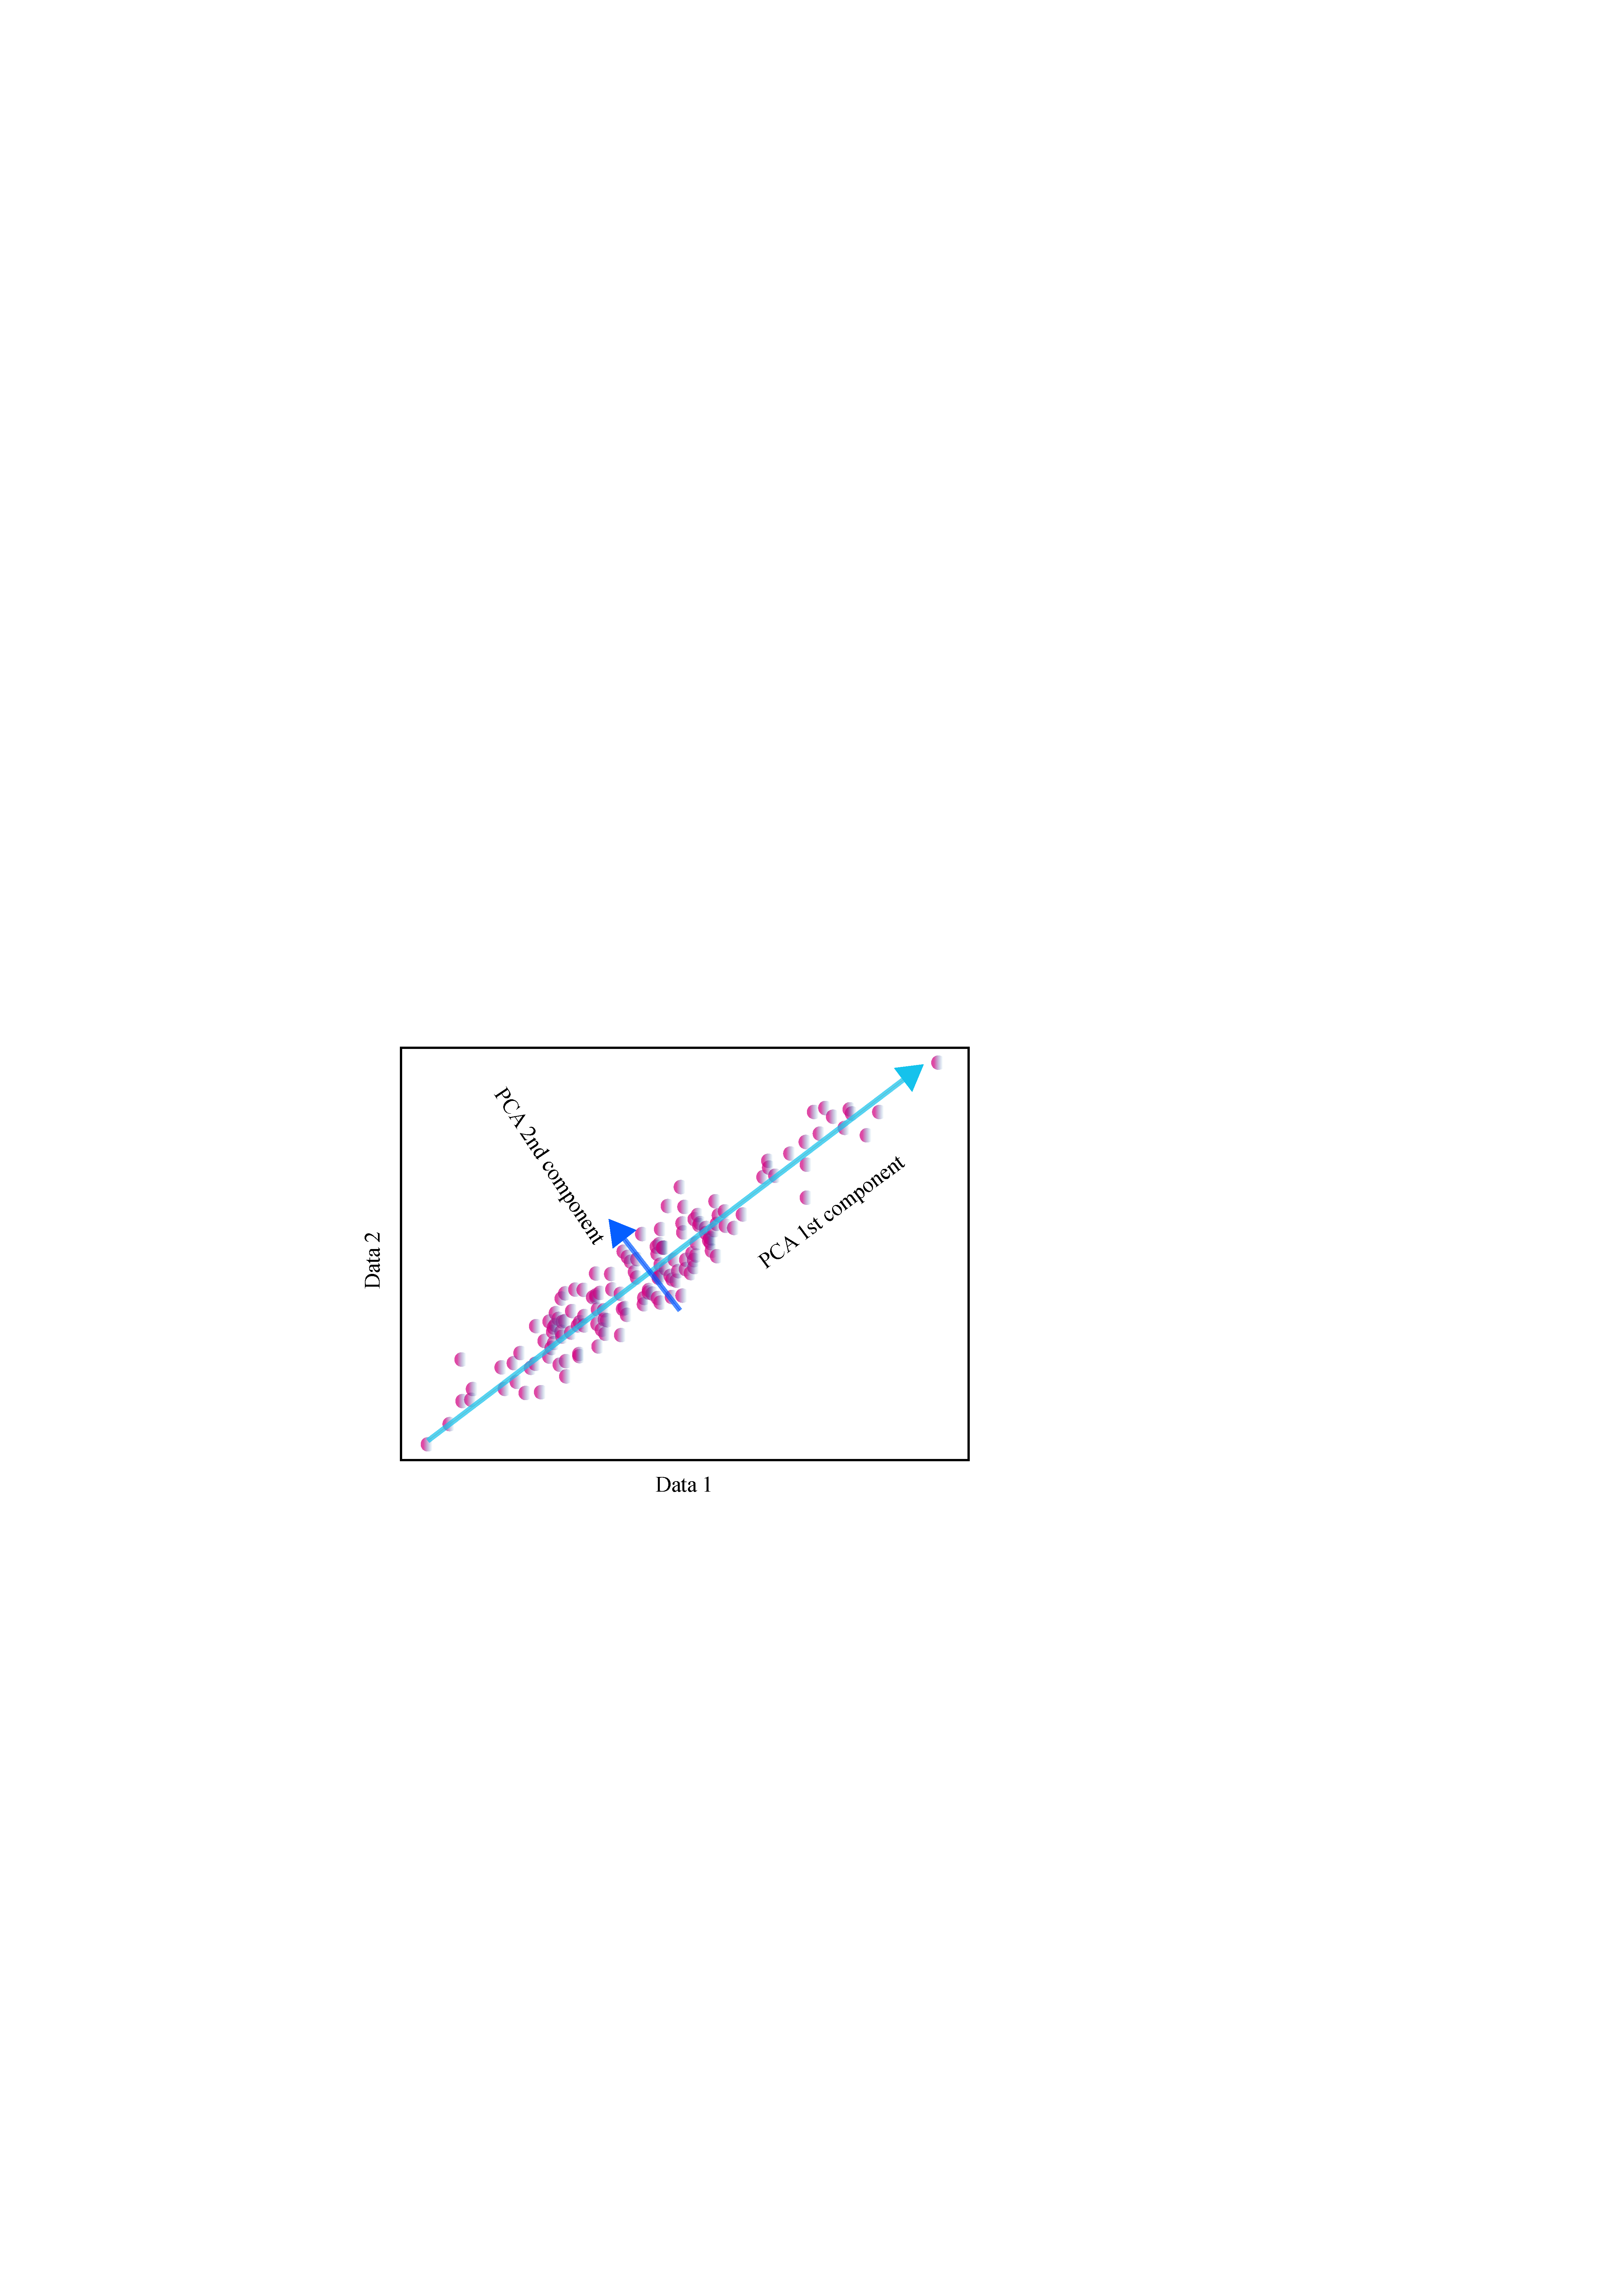
\includegraphics[width=\linewidth]{figures/figure-PCA-2D.pdf}
  \caption{\textit{An example of PCA process on a two-dimensional data}}
  \label{fig: PCA-2D}
\end{marginfigure}





 By retaining only those $N'$ principal components with the highest variance, the model output $\boldsymbol{Y}$ can then be compressed to a lower dimensional subspace $\boldsymbol{Z}$. 
 \begin{equation}
 \label{eq: PCA-component}
\boldsymbol{Z} =  \boldsymbol{\Phi}^{\mathsf{T}}_{N'}
(\boldsymbol{Y} - \boldsymbol{\mu_{Y}}) \approx \boldsymbol{Z}_{\text{full}}
\end{equation} 
Each realization (\textit{observation sample}) can reduce the number of outputs though  \Cref{eq: PCA-component}. A specific realization $\boldsymbol{x}^{k}$ can be visualized in \Cref{fig: PCA-schematic} based on the selected eigenvectors $ \boldsymbol{\Phi}^{\mathsf{T}}_{N'}$. 
% \begin{figure}[htbp]
%     \centering    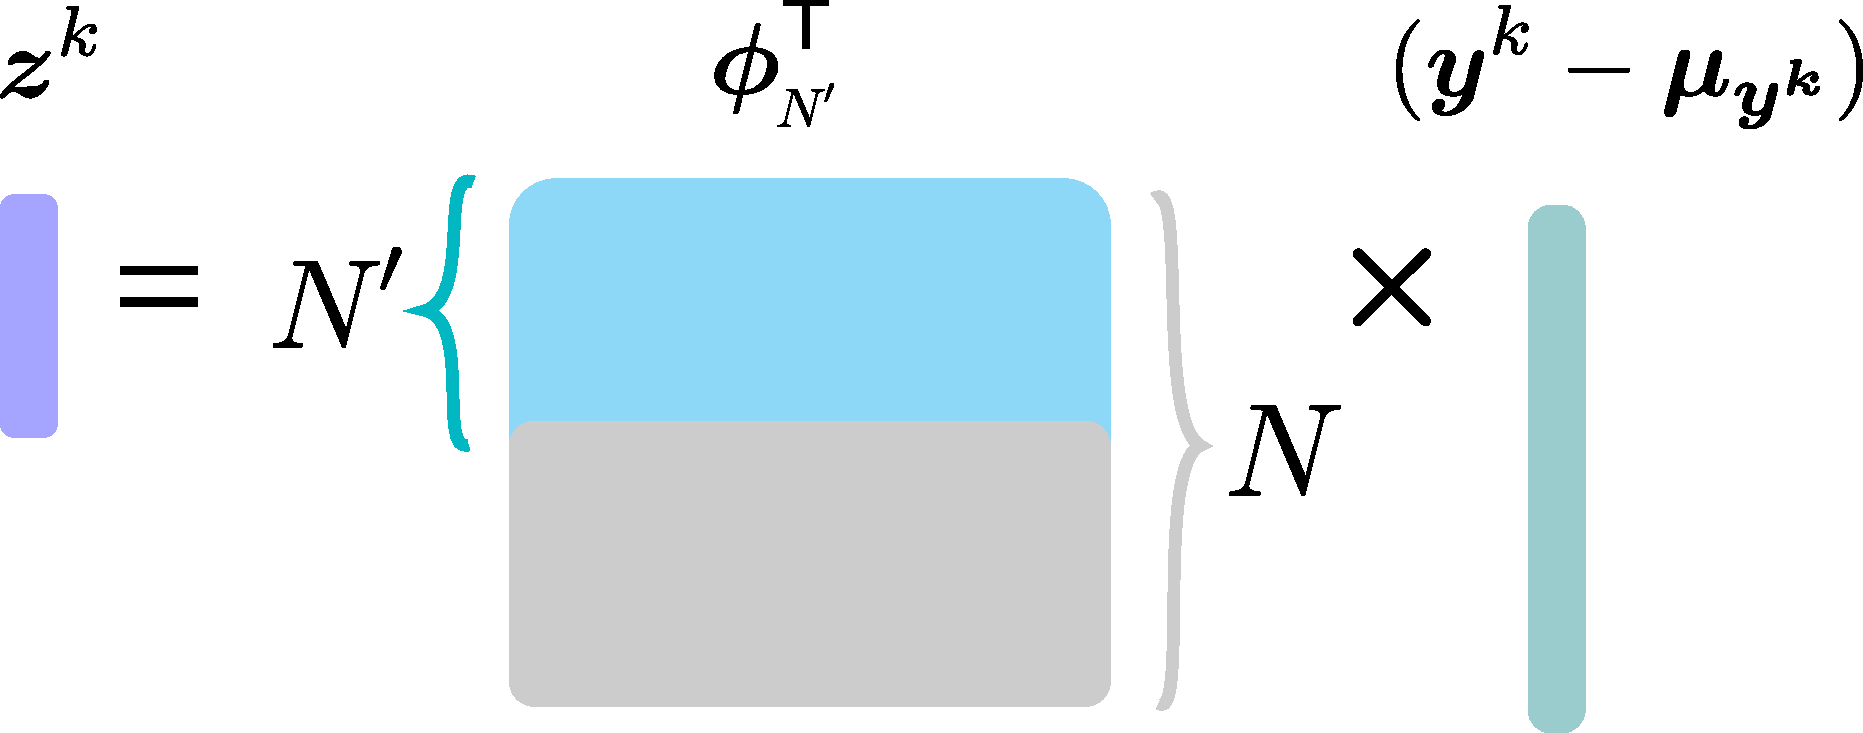
\includegraphics[width=110mm]{figures/figure-PCA-skematic.pdf}
%     \caption{\textit{A visualized realization of data compressing with selected eigenvectors}}
%     \label{fig: PCA-schematic}
% \end{figure}
\begin{marginfigure}%
  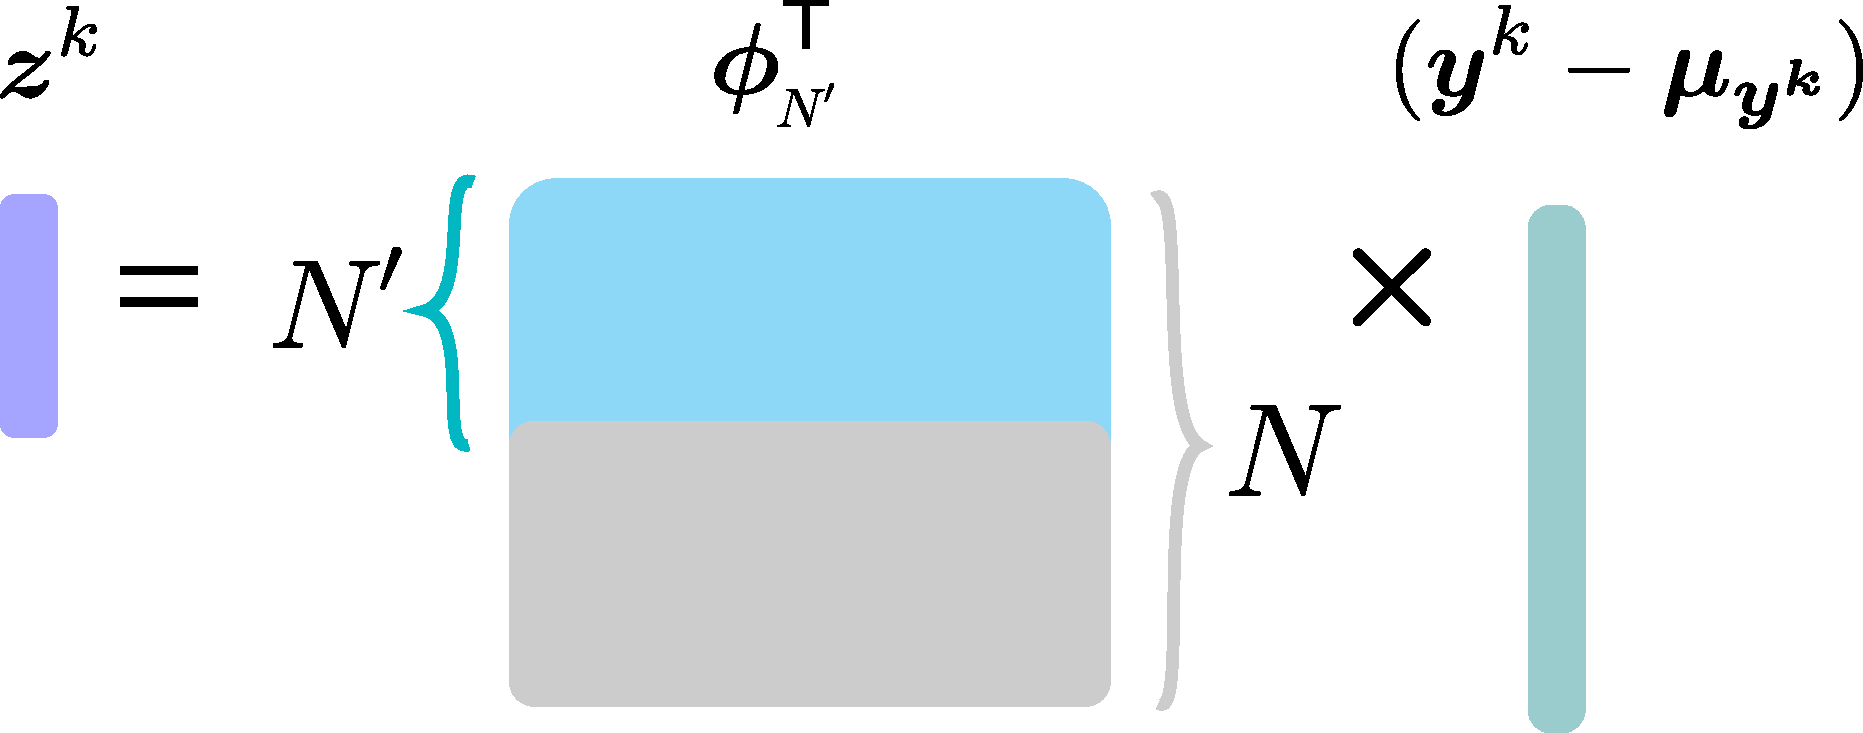
\includegraphics[width=\linewidth]{figures/figure-PCA-skematic.pdf}
  \caption{\textit{A visualized realization of data compressing with selected eigenvectors}}
  \label{fig: PCA-schematic}
\end{marginfigure} All dataset can be then compressed while retaining most of the total variation by:
\begin{equation}
    \label{PCA-components_expression_Z}
    \boldsymbol{z} = 
\begin{bmatrix}
({\boldsymbol{z}^{1}})^{\mathsf{T}} \\
({\boldsymbol{z}^{2}})^{\mathsf{T}} \\
\cdots \\
({\boldsymbol{z}^{K}})^{\mathsf{T}} 
\end{bmatrix}
=
\begin{bmatrix}
z_{1}^{1} & z_{2}^{1} & \cdots & z_{N'}^{1} \\
z_{1}^{2} & z_{2}^{2} & \cdots & z_{N'}^{2}  \\
\vdots & \vdots & \ddots & \vdots \\
z_{1}^{K} & z_{2}^{K} & \cdots & z_{N'}^{K}
\end{bmatrix} 
\end{equation}



 The selection of the number $N'$ is determined such that $\sum_{i=1}^{N'} \lambda_{i} = 
(1-\varepsilon_{\text{DR}}^{threshold})\sum_{i=1}^{N} \lambda_{i}$, where $\varepsilon_{\text{DR}}^{threshold}$ is a prespecified threshold. An adequate number of principal components is to represent the system in an optimal way. If few PCs are selected than required, a poor model will be obtained. On the contrary, if more PCs than necessary are selected, the model will still face the pressure from high dimensionality. In real high-dimensional data outputs, it may also encounter the problems of over-parameterized and will include noise. To avoid these problems, several criteria for selecting the optimum number of PCs were proposed such as scree plot, explain-variance, permutation test, cross-validation and variance of reconstruction error \cite{valle1999,saccenti2015,qin2000,mnassri2010}. With a suitable threshold and choosing criteria, the original space can be reconstructed as $\boldsymbol{Y}^{Re}$ through its optimum $N'$ principal components using \Cref{eq: PCA-reconstruct}:
\begin{equation}
\label{eq: PCA-reconstruct}
\boldsymbol{Y} 
=\boldsymbol{\mu_{Y}} + 
\sum_{i=1}^{N} \boldsymbol{z}_{i}\boldsymbol{\phi}_{i}
\approx \boldsymbol{Y}^{Re} 
= \boldsymbol{\mu_{Y}} + 
\sum_{i=1}^{N'} \boldsymbol{z}_{i}\boldsymbol{\phi}_{i}
\end{equation}



Similar to PCA, most DR techniques share the same ingredients as illustrated in \Cref{fig: PCA-flowchart}: (1) calculate the reduced latent spaces $\boldsymbol{Z} $ (e.g., principal components in PCA) and (2) based on a predefined threshold $\varepsilon_{\text{DR}}^{threshold}$ and transform process $\mathcal{T}_{DR}^{-1}$, the outputs $\boldsymbol{Y}^{Re}$ can be reconstructed. A suitable number of latent spaces $N'$ can be retained. While PCA is a highly effective and powerful compression tool, the main idea of PCA is still based on linear decomposition. As data complexity increases, the limitations of PCA become apparent. In such cases, more advanced DR techniques, like \textit{MDS}, \textit{kPCA}, and \textit{autoencoder}, come into play.
\begin{figure}
  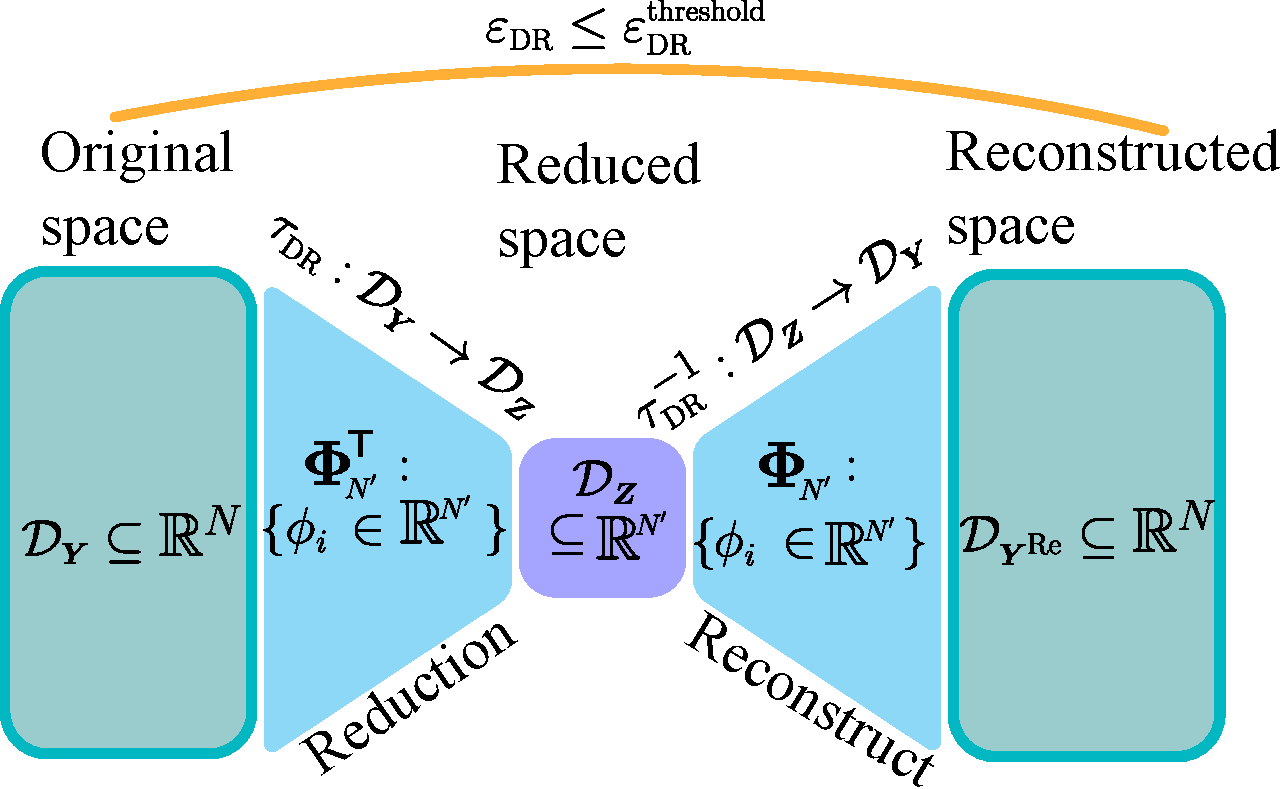
\includegraphics{figures/figure-PCA-flowchart.pdf}
%  \checkparity This is an \pageparity\ page.%
  \caption{\textit{DR-flowchart}}
  \label{fig: PCA-flowchart}
  \setfloatalignment{b}
\end{figure}


\bibliography{sample-handout}
\bibliographystyle{plainnat}



\end{document}
